%Este trabalho está licenciado sob a Licença Atribuição-CompartilhaIgual 4.0 Internacional Creative Commons. Para visualizar uma cópia desta licença, visite http://creativecommons.org/licenses/by-sa/4.0/deed.pt_BR ou mande uma carta para Creative Commons, PO Box 1866, Mountain View, CA 94042, USA.

\chapter{Método de elementos finitos em 1D}\label{cap_mef1d}
\thispagestyle{fancy}

\section{Fundamentos preliminares}\label{cap_mef1d_sec_fund}

Seja dado um intervalo $I = [x_0, x_1]\subset\mathbb{R}$, $x_0\neq x_1$. O espaço vetorial das funções lineares em $I$ é definido por
\begin{equation}
  P_1(I) := \{v:~v(x)=c_0+c_1x,~x\in I,~c_0,c_1\in\mathbb{R}\}.
\end{equation}
Observamos que dado $v\in P_1(I)$, temos que $v$ é unicamente determinada pelos valores $\alpha_0=v(x_0)$ e $\alpha_1=v(x_1)$. Como consequência, existe exatamente uma única função $v\in P_1(I)$ para quaisquer dados valores $\alpha_0$ e $\alpha_1$. Desta observação, introduzimos a chamada base nodal $\{\varphi_0, \varphi_1\}$ para $P_1(I)$, definida por
\begin{equation}
  \varphi_j(x_i) = \left\{
    \begin{array}{ll}
      1 &, i=j,\\
      0 &, i\neq j
    \end{array}
\right.,
\end{equation}
com $i,j=0,1$. Com esta base, toda função $v\in P_1(I)$ pode ser escrita como uma combinação linear das funções $\varphi_0$ e $\varphi_1$ com coeficientes $\alpha_0$ e $\alpha_1$ (\pmb{graus de liberdade}\index{graus de liberdade}), i.e.
\begin{equation}
  v(x) = \alpha_0\varphi_0(x) + \alpha_1\varphi_1(x_1).
\end{equation}
Além disso, observamos que
\begin{equation}
  \varphi_0(x) = \frac{x_1-x}{x_1-x_0},\quad \varphi_1(x)=\frac{x-x_0}{x_1-x_0}.
\end{equation}

Uma extensão do espaço $P_1(I)$ é o espaço das funções lineares por partes. Dado $I = [l_0, l_1]$, $l_0\neq l_1$, consideremos uma partição (\pmb{malha}\index{malha}) de $I$ com $n+1$ pontos $\mathcal{I} = \{l_0=x_0, x_1, \dotsc, x_n=l_1\}$ e, portanto, com $n$ subintervalos $I_i=[x_{i-1}, x_{i}]$ de comprimento $h_i = x_i-x_{i-1}$, $i=1, 2, \dotsc, n$. Na malha $\mathcal{I}$ definimos o seguinte espaço das funções lineares por partes
\begin{equation}
  V_h := \{v:~v\in C^0(\mathcal{I}),~v|_{I_i}\in P_1(I_i),~i=1,2,\dotsc,n\}.
\end{equation}
Observamos que toda função $v\in V_h$ é unicamente determinadas por seus valores nodais $\{\alpha_i = v(x_i)\}_{i=0}^n$. Reciprocamente, todo conjunto de valores nodas $\{\alpha_i\}_{i=0}^n$ determina unicamente uma função $v\in V_h$. Desta observação, temos que os valores nodais determinam os graus de liberdade com a base nodal $\{\varphi_j\}_{j=0}^n$ para $V_h$ definida por
\begin{equation}
  \varphi_j(x_i) = \left\{
    \begin{array}{ll}
      1 &, i=j,\\
      0 &, i\neq j
    \end{array}
\right.,
\end{equation}
com $i,j=0,1,\dotsc,n$. Podemos verificar que
\begin{equation}
  \varphi_i(x) = \left\{
    \begin{array}{ll}
      (x-x_{i-1})/h_i &, x\in I_i,\\
      (x_{i+1}-x)/h_{i+1} &, x\in I_{i+1},\\
      0 &, \text{noutros casos}
    \end{array}
\right.
\end{equation}
veja, Figura~\ref{fig:baselinear}. É notável que $\phi_i(x)$ tem suporte compacto $I_i\cup I_{i+1}$.

\begin{figure}[h!]
  \centering
  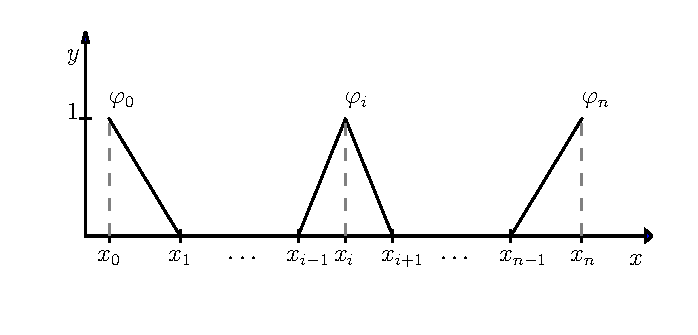
\includegraphics[width=\textwidth]{./cap_mef1d/dados/fig_baselinear/fig_baselinear}
  \caption{Base nodal para o espaço das funções lineares por parte.}
  \label{fig:baselinear}
\end{figure}

\subsection{Interpolação}

A interpolação é uma das técnicas de aproximação de funções. Dada uma função contínua $f$ em $I=[x_0, x_1]$, definimos o \pmb{operador de interpolação linear}\index{operador!interpolação linear} $\pi: C^0(I)\to P_1(I)$ por
\begin{equation}
  \pi f (x) = f(x_0)\varphi_0(x) + f(x_1)\varphi_1(x).
\end{equation}
Observamos que $\pi f$ é igual a $f$ nos nodos $x_0$ e $x_1$. 

\begin{ex}\label{ex:interp_lin}
  A Figura~\ref{fig:ex_interp_lin} ilustra a interpolação da função $f(x)=3\sen(2\pi x)$ no espaço $P_1([1/4, 3/4)]$. Neste caso
  \begin{equation}
    \pi f(x) = f\left(\frac{1}{4}\right)\frac{3/4-x}{1/2} + f\left(\frac{3}{4}\right)\frac{x-1/4}{1/2}.
  \end{equation}

  \begin{figure}[h!]
    \centering
    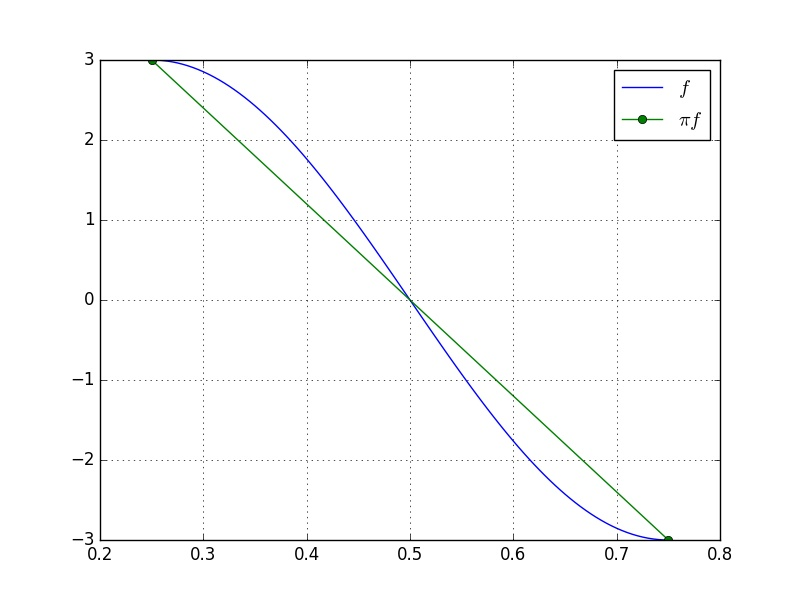
\includegraphics[width=0.8\textwidth]{./cap_mef1d/dados/ex_interp_lin/ex_interp_lin}
    \caption{Interpolação linear de $f(x)=3\sen(2\pi x)$ no espaço $P_1([1/4, 3/4])$.}
    \label{fig:ex_interp_lin}
  \end{figure}

\ifispython
Com o \fenics, podemos computar a função interpolada $\pi f$ com o seguinte \href{https://github.com/phkonzen/notas/blob/master/src/MetodoElementosFinitos/cap_mef1d/dados/ex_interp_lin/ex_interp_lin.py}{código}:
\verbatiminput{./cap_mef1d/dados/ex_interp_lin/ex_interp_lin.py}
\fi
\end{ex}

Agora, vamos buscar medir o erro de interpolação, i.e. $f - \pi f$. Para tanto, podemos usar a norma $L^2$ definida por
\begin{equation}
  \|v\|_{L^2(I)} = \left(\int_i v^2\, dx\right)^{1/2}.
\end{equation}
Lembramos que valem as desigualdades triangular
\begin{equation}
  \|v+w\|_{L^2(I)} \leq \|v\|_{L^2(I)} +  \|w\|_{L^2(I)}
\end{equation}
e a de Cauchy-Schwarz
\begin{equation}\label{eq:Cauchy-Schwarz}
  \int_I vw\,dx \leq \|v\|_{L^2(I)}\|w\|_{L^2(I)},
\end{equation}
para qualquer funções $v,w\in L^2(I)$.

\begin{prop}\normalfont(Erro da interpolação linear)\label{prop:interp_lin}
  O interpolador $\pi f$ satisfaz as estimativas
  \begin{align}
    \|f-\pi f\|_{L^2(I)} &\leq Ch^2\|f''\|_{L^2(I)},\\
    \|(f-\pi f)'\|_{L^2(I)} &\leq Ch\|f''\|_{L^2(I)},
  \end{align}
onde $C$ é uma constante e $h=x_1-x_0$.
\end{prop}
\begin{dem}
  Denotemos o erro de interpolação por $e = f - \pi f$. Do teorema fundamental do cálculo, temos
  \begin{equation}
    e(y) = e(x_0) + \int_{x_0}^y e'(x)\,dx,
  \end{equation}
onde $e(x_0)=f(x_0)-\pi f(x_0) = 0$. Daí, usando a desigualdade de Cauchy-Schwarz~\eqref{eq:Cauchy-Schwarz}, temos
\begin{align}
  e(y) &= \int_{x_0}^y e'\,dx\\
       &\leq \int_{x_0}^y |e'|\,dx\\
       &\leq \int_{I} 1\cdot |e'|\,dx\\
       &\leq \left(\int_{I} 1^2\,dx\right)^{1/2} \left(\int_{I} e'^2\,dx\right)^{1/2}\\
       &= h^{1/2}\left(\int_{I} e'^2\,dx\right)^{1/2},
\end{align}
donde
\begin{equation}
  e(y)^2 \leq h\int_I e'^2\,dx = h\|e'\|_{L^2(I)}^2.
\end{equation}
Então, integrando em $I$ obtemos
\begin{equation}
  \|e\|_{L^2(I)}^2 = \int_I e^2(y)\,dy \leq \int_I h\|e'\|_{L^2(I)}^2\,dy = h^2\|e'\|_{L^2(I)}^2,
\end{equation}
ou seja,
\begin{equation}\label{eq:prop_pif_0}
  \|e\|_{L^2(I)} \leq h\|e'\|_{L^2(I)}.
\end{equation}

Agora, observando que $e(x_0)=e(x_1)=0$, o teorema de Rolle garante a existência de um ponto $\tilde{x}\in I$ tal que $e'(\tilde{x})=0$, donde do teorema fundamental do cálculo e da desigualdade de Cauchy-Schwarz, segue
\begin{align}
  e'(y) &= e'(\tilde{x}) + \int_{\tilde{x}}^y e''\,dx \\
        &= \int_{\tilde{x}}^y e''\,dx\\
        &\leq \int_{I}1\cdot |e''|\,dx\\
        &\leq h^{1/2}\left(\int_I e''^2\right)^{1/2}.
\end{align}
Então, integrando em $I$, obtemos
\begin{equation}\label{eq:prop_pif_1}
  \|e'\|_{L^2(I)}^2 \leq h^2\|e''\|_{L^2(I)}^2,
\end{equation}
a qual, observando que $e'' = f''$, equivale a segunda estimativa procurada, i.e.
\begin{equation}
  \|(f-\pi f)'\|_{L^2(I)} \leq C h \|f''\|_{L^2(I)}.
\end{equation}
Por fim, de \eqref{eq:prop_pif_0} e de \eqref{eq:prop_pif_0}, obtemos a primeira estimativa desejada
\begin{equation}
  \|f - \pi f\|_{L^2(I)} \leq C h^2 \|f''\|_{L^2(I)}.
\end{equation}
\end{dem}

Vamos, agora, generalizar este resultado para a interpolação no espaço $V_h$ das funções lineares por parte. Dada uma função contínua $f$ em $I = [l_0, l_1]$, definimos o operador interpolador $\pi: C^0(I)\to V_h$ na malha $\mathcal{I}$ de $I$ por
\begin{equation}
  \pi f(x) = \sum_{i=0}^{n}f(x_i)\varphi_i(x).
\end{equation}

\begin{ex}\label{ex:interp_linpartes}
  A Figura~\ref{fig:ex_interp_linpartes} ilustra a interpolação da função $f(x)=3\sen(2\pi x)$ no espaço $V_h$ das funções lineares por partes em uma malha uniforme do intervalo $I=[1/4, 3/4]$ com $n=4$ subintervalos ($5$ pontos). 

  \begin{figure}[h!]
    \centering
    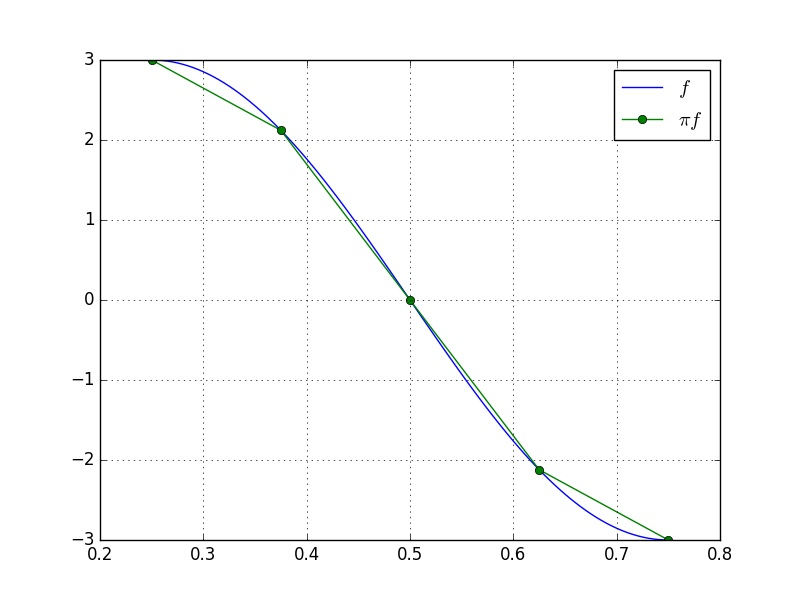
\includegraphics[width=0.8\textwidth]{./cap_mef1d/dados/ex_interp_linpartes/ex_interp_linpartes}
    \caption{Interpolação linear de $f(x)=3\sen(2\pi x)$ no espaço $V_h$ das funções lineares por partes sobre uma malha com $5$ pontos.}
    \label{fig:ex_interp_linpartes}
  \end{figure}

\ifispython
Com o \fenics, podemos computar a função interpolada $\pi f$ com o seguinte \href{https://github.com/phkonzen/notas/blob/master/src/MetodoElementosFinitos/cap_mef1d/dados/ex_interp_linpartes/ex_interp_linpartes.py}{código}:
\verbatiminput{./cap_mef1d/dados/ex_interp_linpartes/ex_interp_linpartes.py}
\fi
\end{ex}

O seguinte resultado fornece uma estimativa do erro de interpolação em relação ao tamanho $h_i$ de cada elemento da malha.

\begin{prop}\label{prop:interp_linpartes}
  O interpolador $\pi f$ satisfaz as estimativas
  \begin{align}
    \|f-\pi f\|_{L^2(I)}^2 &\leq C\sum_{i=1}^n h_i^4\|f''\|_{L^2(I)}^2,\\
    \|(f-\pi f)'\|_{L^2(I)}^2 &\leq C\sum_{i=1}^n h_i^2\|f''\|_{L^2(I)}^2.\\
  \end{align}
\end{prop}
\begin{dem}
  Ambas desigualdades seguem da desigualdade triangular e da Proposição~\ref{prop:interp_lin}. Por exemplo, para a primeira desigualdade, temos
  \begin{align}
    \|f - \pi f\|_{L^2(I)}^2 &\leq \sum_{i=1}^n \|f - \pi f\|_{L^2(I_i)}^2\\
    &\leq \sum_{i=1}^n Ch_i^4 \|f''\|_{L^2(I_i)}^2.
  \end{align}
\end{dem}

\subsection{Projeção $L^2$}

Dada uma função $f\in L^2(I)$, definimos o \emph{operador de projeção $L^2$}\index{operador de!projeção $L^2$} $P_h:L^2(I)\to V_h$ por
\begin{equation}\label{eq:proj_def}
  \int_I (f-P_hf)v\,dx=0,\quad\forall v\in V_h.
\end{equation}

Como $V_h$ é um espaço de dimensão finita, a condição \eqref{eq:proj_def} é equivalente a
\begin{equation}\label{eq:proj_def}
  \int_I (f-P_hf)\varphi_i\,dx=0,\quad i=0, 1, \cdots, n,
\end{equation}
onde $\varphi_i$ é a $i$-ésima função base de $V_h$. Além disso, como $P_hf\in V_h$, temos
\begin{equation}
  P_hf = \sum_{j=0}^n\xi_j\varphi_j,
\end{equation}
onde $\xi_j$, $j=0, 1, \dotsc, n$, são $n+1$ incógnitas a determinar. Logo,
\begin{align}
  \int_I (f-P_hf)\varphi_i\,dx=0 &\Leftrightarrow \int_I f\varphi_i\,dx = \int_I P_hf\varphi_i\,dx\\
  &\Leftrightarrow \int_I f\varphi_i\,dx = \int_I \left(\sum_{j=0}^n \xi_j\varphi_j\right)\varphi_i\,dx\\
  &\Leftrightarrow \sum_{j=0}^n \xi_j\int_I\varphi_j\varphi_i\,dx = \int_I f\varphi_i\,dx,\label{eq:proj_siseq}
\end{align}
para $i=0, 1, \dotsc, n$.

Observemos, agora, que \eqref{eq:proj_siseq} consiste em um sistema de $n+1$ equações lineares para as $n+1$ incógnitas $\xi_j$, $j=0, 1, \dotsc, n$. Este, por sua vez, pode ser escrito na seguinte forma matricial
\begin{equation}\label{eq:proj_sis}
  M\xi = b,
\end{equation}
onde $M = [m_{i,j}]_{i,j=0}^{n+1}$ é chamada de matrix de massa
\begin{equation}
  m_{i,j} = \int_I\varphi_j\varphi_i\,dx
\end{equation}
e $b = (b_0, b_1, \dotsc, b_n)$ é chamado de vetor de carregamento
\begin{equation}
  b_i = \int_I f\varphi_i\,dx.
\end{equation}

Ou seja, a projeção $L^2$ de $f$ no espaço $V_h$ é
\begin{equation}
  P_hf = \sum_{j=0}^n\xi_j\varphi_j,
\end{equation}
onde $\xi = (\xi_0, \xi_1, \dotsc, \xi_n)$ é solução do sistema \eqref{eq:proj_sis}.

\begin{ex}\label{ex:proj}
  A Figura~\ref{fig:ex_proj} ilustra a projeção $L^2$ da função $f(x)=3\sen(2\pi x)$ no espaço $V_h$ das funções lineares por partes em uma malha uniforme do intervalo $I=[1/4, 3/4]$ com $n=4$ subintervalos ($5$ pontos). 

  \begin{figure}[h!]
    \centering
    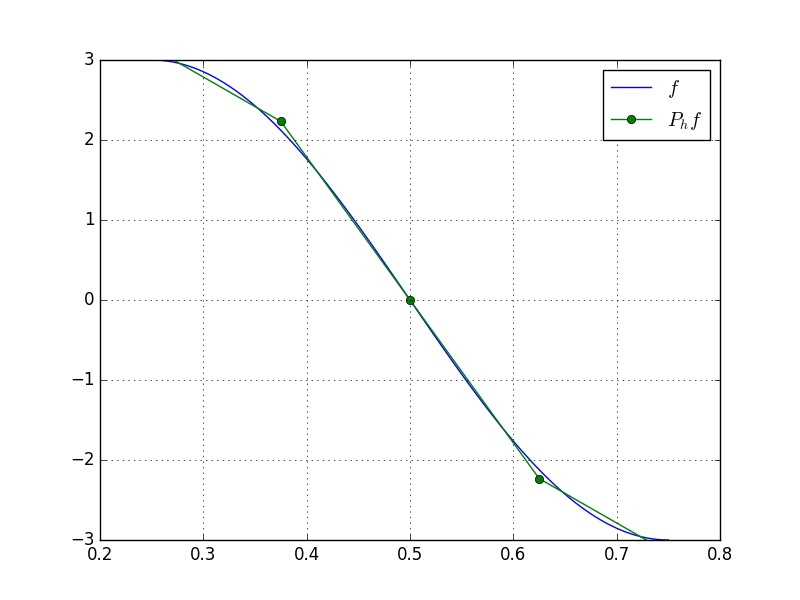
\includegraphics[width=0.8\textwidth]{./cap_mef1d/dados/ex_proj/ex_proj}
    \caption{Projeção $L^2$ de $f(x)=3\sen(2\pi x)$ no espaço $V_h$ das funções lineares por partes sobre uma malha com $5$ pontos.}
    \label{fig:ex_proj}
  \end{figure}

\ifispython
Com o \fenics, podemos computar $P_h f$ com o seguinte \href{https://github.com/phkonzen/notas/blob/master/src/MetodoElementosFinitos/cap_mef1d/dados/ex_proj/ex_proj.py}{código}:
\verbatiminput{./cap_mef1d/dados/ex_proj/ex_proj.py}
\fi
\end{ex}

\emconstrucao

\subsection{Exercícios}

\begin{exer}
  Faça um código para verificar as estimativas da Proposição~\ref{prop:interp_lin} no caso da interpolação da função $f(x) = 3\sen(2\pi x)$ no espaço $P_1$ das funções lineares.
\end{exer}

\begin{exer}
  Faça um código para verificar as estimativas da Proposição~\ref{prop:interp_linpartes} no caso da interpolação da função $f(x) = 3\sen(2\pi x)$ no espaço $V_h$ das funções lineares por partes.
\end{exer}

\emconstrucao